\section{平面镜成像}\label{sec:1-3}

\begin{wrapfigure}[11]{r}{5.5cm}
    \centering
    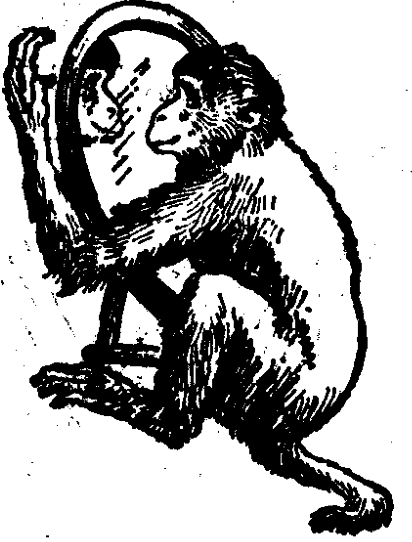
\includegraphics[width=4cm]{../pic/czwl2-ch1-6}
    \caption{}\label{fig:1-6}
\end{wrapfigure}


猴子从镜子里看到了一只猴子,想去镜后抓住它。结果什么也抓不着(图 \ref{fig:1-6})。
原来,聪明的猴子不懂得镜子里的猴子就是它自己的像。

日常生活里常用的镜子表面是平的,叫做\textbf{平面镜}。
这一节,我们就来研究平面镜成像。


在图 \ref{fig:1-7} 里,光从发光点 $S$ 发出,光线 $SA$、$SC$ 被镜面反射后,
分别沿 $AB$、$CD$ 的方向射进我们的眼睛里。
发光点虽然在 $S$,可是我们逆着反射光线的方向看去,
就觉得发光点好象在镜子后面的 $S_1$ 处,$S_1$ 就是发光点 $S$ 的像。
显然,实际上光线不是来自 $S_1$ 点,镜子后面也不存在发光点 $S_1$,所以这个像是\textbf{虚像}。

镜子前面的物体可以看成是由许多点组成的,每个点在镜子里都有一个像,这些像就组成物体的像。
物体在平面镜里的像也是虚像。

\begin{figure}[htbp]
    \centering
    \begin{minipage}{7cm}
    \centering
    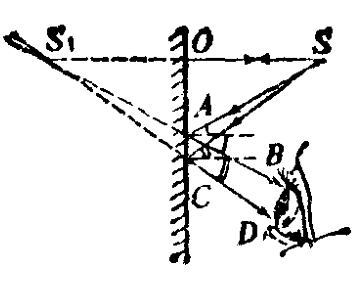
\includegraphics[width=4cm]{../pic/czwl2-ch1-7}
    \caption{}\label{fig:1-7}
    \end{minipage}
    \qquad
    \begin{minipage}{7cm}
    \centering
    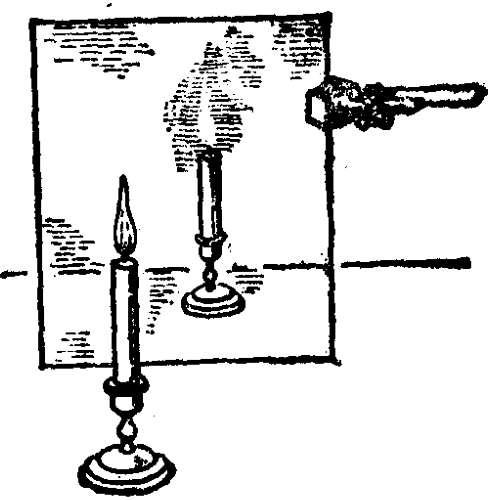
\includegraphics[width=5cm]{../pic/czwl2-ch1-8}
    \caption{}\label{fig:1-8}
    \end{minipage}
\end{figure}


在桌面上竖直地立一块玻璃板,玻璃板的前面点一支蜡烛(图 \ref{fig:1-8}),
就会看到玻璃板跟平面镜相似,在它的后面有蜡烛的像。
再拿一支同样的,不过没有点着的蜡烛,把它放在玻璃板的后面,
并且前后左右移动它,直到从玻璃前面的各处看来,这支蜡烛也好象点着似的为止。
这说明,没有点着的蜡烛恰好在点着的蜡烛的虚像的位置上,而且它们的大小相等;
如果测量下,还会发现,两支蜡烛的连线跟玻璃板垂直,它们到玻璃板的距离相等。

可见,\textbf{物体在平面镜里成的是虚像;像和物体的大小相等,
它们的连线跟镜面垂直,它们到镜面的距离相等}。

光滑的金属面,平静的水面,都具有平面镜的作用,能够形成清晰的像。
在玻璃发明以前,古代的人就用磨光的铜盘做镜子。
平静的水面能够清楚地映出岸上的景物,造成美丽的景色(\hyperref[fig:pic1]{彩图1}), 也是平面镜成像的结果。

\begin{figure}[htbp]
    \centering
    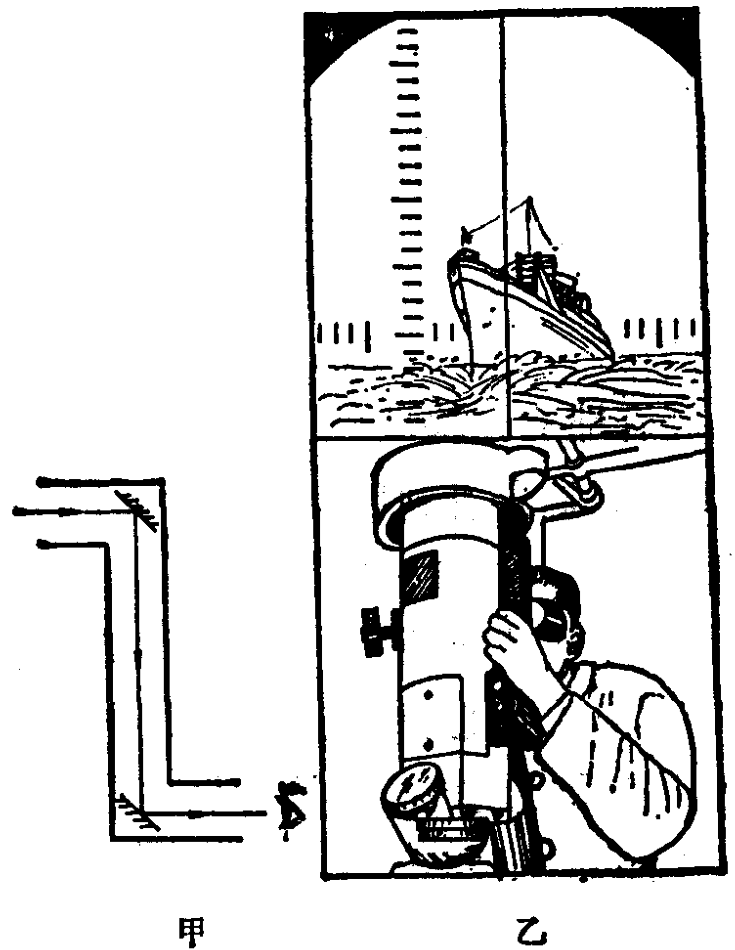
\includegraphics[width=0.6\textwidth]{../pic/czwl2-ch1-9}
    \caption{潜望镜}\label{fig:1-9}
\end{figure}

平面镜还广泛安装在各种仪器中,用来改变光线的方向。
潜望镜就是其中的一个例子,最简单的潜望镜(图 \ref{fig:1-9} 甲)是在管子的上方和下方拐角处各装一块平面镜,
两块平面镜互相平行,都跟水平方向成 $45^\circ$ 角。
高处物体沿水平方向射入镜筒中的光线经两块平面镜反射后仍沿水平方向射出,进入观察者的眼中。
这样就可以从潜望镜中看见被掩蔽物挡住的物体。
潜望镜可以用在战壕里,潜水艇里,观察外面的情况(图 \ref{fig:1-9} 乙)。

平面镜成像的现象有时对我们不利。
例如,汽车在夜间行驶的时候,假如车内开着灯,司机前面的玻璃窗就会象平面镜那样,
反射车内物体投射来的光,使司机看见车内物体的像,而妨碍看清前面的道路。
因此,汽车在夜间行驶,车内不开灯,以保证行车安全。

